% -*- TeX -*-
\documentclass{beamer}

\usepackage{tikz}
\usetikzlibrary{shapes,calc}

\title{Crustal Deformation Modeling Workshop}
\subtitle{Introduction and Overview of Tutorials}
\author{Brad Aagaard}
\institute{
\includegraphics[scale=0.4]{../../logos/cig_blackfg}%\\
%Username: guest-cfem\\
%Password: 6jjcrjnm
}
\date{June 23--27, 2014}


% ---------------------------------------------------- CUSTOMIZATION
\newcommand{\thispdfpagelabel}[1]{}
\newcommand{\important}[1]{{\bf\color{red}#1}}
\usetheme{CIG}

% --------------------------------------------------------- DOCUMENT
\begin{document}

% ------------------------------------------------------------ SLIDE
\maketitle

% ------------------------------------------------------------ SLIDE
\begin{frame}
  \frametitle{PyLith v2.0.1 available}
  \summary{}
  
  Wireless: Stanford (Guest), Username: CDMJune2014, Password:
  CDMJune2014
  \vfill
  \important{PyLith v2.0.1 available}\\
  Fixes several issues associated with CUBIT/Trelis compatibility.
  \vfill
  
\end{frame}


% ------------------------------------------------------------ SLIDE
\begin{frame}
  \frametitle{Daily Notices}
  \summary{}
  
  Wireless: Stanford (Guest), Username: CDMJune2014, Password:
  CDMJune2014
  \vfill
  \important{Mon: PyLith v2.0.1 available}\\
  Fixes several issues associated with CUBIT/Trelis compatibility.
  \vfill
  \important{Tue: Debugging example files available}\\
  {\tt wiki.geodynamics.org} $\rightarrow$ PyLith $\rightarrow$ Additional Examples
  \vfill
  
\end{frame}


% ========================================================== SECTION
\section{Sunrise: 5:45am}
\subsection{Sunset: 8:30pm}

% ------------------------------------------------------------ SLIDE
\begin{frame}
  \frametitle{Welcome to California}
  \summary{Wireless: Stanford (Guest), Username: CDMJune2014, Password: CDMJune2014}
  
  \begin{center}
    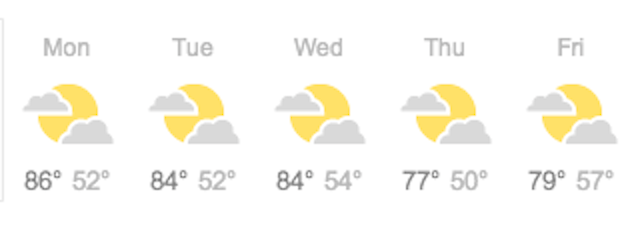
\includegraphics[scale=0.5]{figs/weather}
  \end{center}
  
\end{frame}


% ========================================================== SECTION
\section{Introduction}
\subsection{Agenda}

% ------------------------------------------------------------- LOGO
\logo{
\includegraphics[height=4.5ex]{../../logos/cig_blackfg}}

% ------------------------------------------------------------ SLIDE
\begin{frame}
  \frametitle{Agenda}
  \summary{}
  
  \definecolor{yellow}{rgb}{1.0, 1.0, 0.45} % 255/255/115
\definecolor{dkyellow}{rgb}{0.9, 0.9, 0.0} % % 230/230/0

\definecolor{ltorange}{rgb}{1.0, 0.74, 0.41} % 255/188/105
\definecolor{orange}{rgb}{0.96, 0.50, 0.0} % 246/127/0

\definecolor{ltred}{rgb}{1.0, 0.25, 0.25} % 255/64/64
\definecolor{red}{rgb}{0.79, 0.00, 0.01} % 201/0/3

\definecolor{ltpurple}{rgb}{0.81, 0.57, 1.00} % 206/145/255
\definecolor{purple}{rgb}{0.38, 0.00, 0.68} % 97/1/175

\definecolor{ltblue}{rgb}{0.2, 0.73, 1.0} % 51/187/255
\definecolor{blue}{rgb}{0.12, 0.43, 0.59} % 30/110/150

\definecolor{ltltgreen}{rgb}{0.7, 1.00, 0.7} % 96/204/14
\definecolor{ltgreen}{rgb}{0.37, 0.80, 0.05} % 96/204/14
\definecolor{green}{rgb}{0.23, 0.49, 0.03} % 59/125/8
  
\definecolor{dkslate}{rgb}{0.18, 0.21, 0.28} % 47/53/72
\definecolor{mdslate}{rgb}{0.45, 0.50, 0.68} % 114/127/173
\definecolor{ltslate}{rgb}{0.85, 0.88, 0.95} % 216/225/229


\tikzstyle{days} = [rectangle, 
                    text width=15mm,
                    text centered,
                    minimum height=2em,
                    thin,
                    font=\bfseries,
                    draw=dkyellow!80!black,
                    top color=yellow,
                    bottom color=dkyellow]
\tikzstyle{game} = [rectangle, 
                      draw=green!80!black,
                      top color=ltgreen!20!white,
                      bottom color=green]
\tikzstyle{break} = [rectangle, 
                      draw=blue!80!black,
                      top color=ltblue!20!white,
                      bottom color=blue]

\begin{center}
\begin{tikzpicture}[scale=0.75, transform shape,
  node distance=6.0em,
  thick]

% Reference points
\coordinate (o1) at (0mm,0mm);
\coordinate (o2) at (+25mm,0mm);
\coordinate (o3) at (+50mm,0mm);
\coordinate (o4) at (+75mm,0mm);
\coordinate (o5) at (+100mm,0mm);


  % Days
  \node (mon) [days] at ($(o1)+(8.5mm,0mm)$) {Mon};
  \node (tue) [days] at ($(o2)+(8.5mm,0mm)$) {Tue};
  \node (wed) [days] at ($(o3)+(8.5mm,0mm)$) {Wed};
  \node (thu) [days] at ($(o4)+(8.5mm,0mm)$) {Thu};
  \node (fri) [days] at ($(o5)+(8.5mm,0mm)$) {Fri};

  % Mon
  \node (monb1) [break, below of=mon, yshift=+3.5em] {Breakfast};
  \node (mong1) [game, below of=monb1, yshift=+3.5em] {AUS v ESP};
  \node (mong2) [game, below of=mong1, yshift=+4.3em] {NED v CHI};
  \node (monb2) [break, below of=mong2, yshift=+3.5em] {Lunch};
  \node (mong3) [game, below of=monb2, yshift=+3.5em] {CMR v BRA};
  \node (mong4) [game, below of=mong3, yshift=+4.3em] {CRO v MEX};

  % Tue
  \node (tueb1) [break, below of=tue, yshift=+3.5em] {Breakfast};
  \node (tueg1) [game, below of=tueb1, yshift=+3.5em] {CSC v ENG};
  \node (tueg2) [game, below of=tueg1, yshift=+4.3em] {ITA v URU};
  \node (tueb2) [break, below of=tueg2, yshift=+3.5em] {Lunch};
  \node (tueg3) [game, below of=tueb2, yshift=+3.5em] {GRE v CIV};
  \node (tueg4) [game, below of=tueg3, yshift=+4.3em] {JAP v COL};

  % Wed
  \node (wedb1) [break, below of=wed, yshift=+3.5em] {Breakfast};
  \node (wedg1) [game, below of=wedb1, yshift=+3.5em] {NIG v ARG};
  \node (wedg2) [game, below of=wedg1, yshift=+4.3em] {BIH v IRN};
  \node (wedb2) [break, below of=wedg2, yshift=+3.5em] {Lunch};
  \node (wedg3) [game, below of=wedb2, yshift=+3.5em] {HON v SUI};
  \node (wedg4) [game, below of=wedg3, yshift=+4.3em] {ECU v FRA};

  % Thu
  \node (thub1) [break, below of=thu, yshift=+3.5em] {Breakfast};
  \node (thug1) [game, below of=thub1, yshift=+3.5em] {USA v GER};
  \node (thug2) [game, below of=thug1, yshift=+4.3em] {POR v GHA};
  \node (thub2) [break, below of=thug2, yshift=+3.5em] {Lunch};
  \node (thug3) [game, below of=thub2, yshift=+3.5em] {ALG v RUS};
  \node (thug4) [game, below of=thug3, yshift=+4.3em] {KOR v BEL};

  % Fri
  \node (frib1) [break, below of=fri, yshift=+3.5em] {Breakfast};
  \node (frig1) [game, below of=frib1, yshift=+3.5em] {TBD};
  \node (frib2) [break, below of=frig1, yshift=+1.8em] {Lunch};

\end{tikzpicture}
\end{center}



\end{frame}


% ------------------------------------------------------------ SLIDE
\begin{frame}
  \frametitle{Overview of Tutorials}
  \summary{}
  
  \definecolor{yellow}{rgb}{1.0, 1.0, 0.45} % 255/255/115
\definecolor{dkyellow}{rgb}{0.9, 0.9, 0.0} % % 230/230/0

\definecolor{ltorange}{rgb}{1.0, 0.74, 0.41} % 255/188/105
\definecolor{orange}{rgb}{0.96, 0.50, 0.0} % 246/127/0

\definecolor{ltred}{rgb}{1.0, 0.25, 0.25} % 255/64/64
\definecolor{red}{rgb}{0.79, 0.00, 0.01} % 201/0/3

\definecolor{ltpurple}{rgb}{0.81, 0.57, 1.00} % 206/145/255
\definecolor{purple}{rgb}{0.38, 0.00, 0.68} % 97/1/175

\definecolor{ltblue}{rgb}{0.2, 0.73, 1.0} % 51/187/255
\definecolor{blue}{rgb}{0.12, 0.43, 0.59} % 30/110/150

\definecolor{ltltgreen}{rgb}{0.7, 1.00, 0.7} % 96/204/14
\definecolor{ltgreen}{rgb}{0.37, 0.80, 0.05} % 96/204/14
\definecolor{green}{rgb}{0.23, 0.49, 0.03} % 59/125/8
  
\definecolor{dkslate}{rgb}{0.18, 0.21, 0.28} % 47/53/72
\definecolor{mdslate}{rgb}{0.45, 0.50, 0.68} % 114/127/173
\definecolor{ltslate}{rgb}{0.85, 0.88, 0.95} % 216/225/229


\tikzstyle{days} = [rectangle, 
                    text centered,
                    thin,
                    draw=dkyellow!80!black,
                    font=\bfseries,
                    top color=yellow,
                    bottom color=dkyellow]
\tikzstyle{admin} = [rectangle, 
                    draw=orange!80!black,
                    top color=ltorange!50!white,
                    bottom color=orange]
\tikzstyle{tutorial} = [rectangle, 
                    draw=green!80!black,
                    top color=ltgreen!20!white,
                    bottom color=green]
\tikzstyle{break} = [rectangle, 
                    draw=blue!80!black,
                    top color=ltblue!20!white,
                    bottom color=blue]
\tikzstyle{tinker} = [rectangle, 
                      draw=ltpurple!80!black,
                      top color=ltpurple!20!white,
                      bottom color=purple!70!white!100]

\begin{center}
\begin{tikzpicture}[scale=0.75, transform shape,
  node distance=2.0em,
  text width=55mm,
  thick]
% Reference points
\coordinate (o1) at (0mm,0mm);
\coordinate (o2) at (+65mm,0mm);

% Days
\node[days] (mon) at ($(o1)$) {Mon};
\node[days] (tue) at ($(o2)$) {Tue};

% Mon
\node[tutorial, below of=mon] (relax_intro) {Relax: Intro}; % relax 45min
\node[tutorial, below of=relax_intro] (pylith_intro) {PyLith: Overview}; % pylith 30min
\node[tutorial, below of=pylith_intro] (cubit_intro) {CUBIT: Overview}; % cubit 30min

\node[break, below of=cubit_intro] (break_mon_am) {Break}; % break 15min

\node[tutorial, below of=break_mon_am] (pylith_subduction) {PyLith: 2-D Subduction Zone}; % pylith 2hrs

\node[break, below of=pylith_subduction] (lunch_mon) {Lunch}; % lunch 45min
\node[tinker, below of=lunch_mon] (tinker_mon_A) {Tinker Time}; % tinker 90min
\node[break, below of=tinker_mon_A] (break_mon_pm) {Break}; % break 30min

\node[tutorial, below of=break_mon_pm] (pylith_friction) {PyLith: Intro to Friction}; % pylith 90min
\node[tutorial, below of=pylith_friction] (relax_more) {Relax: More Examples}; % relax 45min
\node[tinker, below of=relax_more] (tinker_mon_B) {Tinker Time}; % tinker 45min

% Tue
\node[tutorial, below of=tue] (cubit_nonplanar) {CUBIT: Nonplanar Geometry}; % cubit 85min
\node[tutorial, below of=cubit_nonplanar] (pylith_solver) {PyLith: Solver Options}; % pylith 45min

\node[break, below of=pylith_solver] (break_tue_am) {Break}; % break 15min

\node[tutorial, below of=break_tue_am] (pylith_afterslip) {PyLith: Frictional Afterslip}; % pylith 30min
\node[tutorial, below of=pylith_afterslip] (pylith_dynrup) {PyLith: Dynamic Rupture}; % pylith 60min

\node[break, below of=pylith_dynrup] (lunch_tue) {Lunch}; lunch 60min
\node[tinker, below of=lunch_tue] (tinker_tue_A) {Tinker Time}; % tinker 90min
\node[break, below of=tinker_tue_A] (break_tue_pm) {Break}; % break 30min

\node[tutorial, below of=break_tue_pm] (pylith_greensfns) {PyLith: Green's Functions}; % pylith 105min
\node[tinker, below of=pylith_greensfns] (tinker_tue_B) {Tinker Time}; % tinker 75min


\end{tikzpicture}
\end{center}


\end{frame}


% ========================================================== SECTION
\subsection{Software}

% ------------------------------------------------------------ SLIDE
\begin{frame}
  \frametitle{Workflow}
  \summary{}

  \usetikzlibrary{arrows,shapes}
\definecolor{yellow}{rgb}{1.0, 1.0, 0.45} % 255/255/115
\definecolor{dkyellow}{rgb}{0.9, 0.9, 0.0} % % 230/230/0

\definecolor{ltorange}{rgb}{1.0, 0.74, 0.41} % 255/188/105
\definecolor{orange}{rgb}{0.96, 0.50, 0.0} % 246/127/0

\definecolor{ltred}{rgb}{1.0, 0.25, 0.25} % 255/64/64
\definecolor{red}{rgb}{0.79, 0.00, 0.01} % 201/0/3

\definecolor{ltpurple}{rgb}{0.81, 0.57, 1.00} % 206/145/255
\definecolor{purple}{rgb}{0.38, 0.00, 0.68} % 97/1/175

\definecolor{ltblue}{rgb}{0.2, 0.73, 1.0} % 51/187/255
\definecolor{blue}{rgb}{0.12, 0.43, 0.59} % 30/110/150

\definecolor{ltltgreen}{rgb}{0.7, 1.00, 0.7} % 96/204/14
\definecolor{ltgreen}{rgb}{0.37, 0.80, 0.05} % 96/204/14
\definecolor{green}{rgb}{0.23, 0.49, 0.03} % 59/125/8
  
\definecolor{dkslate}{rgb}{0.18, 0.21, 0.28} % 47/53/72
\definecolor{mdslate}{rgb}{0.45, 0.50, 0.68} % 114/127/173
\definecolor{ltslate}{rgb}{0.85, 0.88, 0.95} % 216/225/229

\tikzstyle{phase} = [rectangle, 
                      draw=dkyellow!80!black,
                      top color=yellow,
                      bottom color=dkyellow]
\tikzstyle{cig} = [rectangle, 
                      rounded corners=0.5em,
                      draw=orange!80!black,
                      top color=ltorange!50!white,
                      bottom color=orange]
\tikzstyle{open} = [rectangle, 
                      rounded corners=0.5em,
                      draw=green!80!black,
                      top color=ltgreen!20!white,
                      bottom color=green]
\tikzstyle{free} = [rectangle, 
                      rounded corners=0.5em,
                      draw=blue!80!black,
                      top color=ltblue!20!white,
                      bottom color=blue]
\tikzstyle{commercial} = [rectangle, 
                      rounded corners=0.5em,
                      draw=ltred!80!black,
                      top color=ltred!20!white,
                      bottom color=red!70!white!100]
\tikzstyle{available} = [thick, color=black]
\tikzstyle{planned} = [thick, dashed, color=mdslate]


\begin{center}
\begin{tikzpicture}[scale=0.75, transform shape,
  node distance=3.0em,
  text width=6em, text centered, minimum height=2em, thick]

  % Phases
  \node (structure) [phase] {Geologic Structure};
  \node (meshing) [phase, right of=structure, xshift=6em] {Mesh Generation};
  \node (physics) [phase, right of=meshing, xshift=6em] {Physics Code};
  \node (viz) [phase, right of=physics, xshift=6em] {Visualization};

  % Geologic structure
  \node (gocad) [commercial, below of=structure] {Gocad};
  \node (earthviz) [commercial, below of=gocad] {Earth Vision};

  % Mesh generation
  \node (cubit) [commercial, below of=meshing] {CUBIT};
  \node (lagrit) [free, below of=cubit] {LaGriT};
  \node (tetgen) [open, below of=lagrit] {TetGen};
  \node (gmsh) [open, below of=tetgen] {Gmsh};

  % Physics code
  \node (pylith) [cig, below of=physics] {PyLith};
  \node (relax) [cig, below of=pylith] {Relax};
  \node (geofest) [free, below of=relax] {GeoFEST};
  \node (abaqus) [commercial, below of=geofest] {Abaqus};

  % Visualization
  \node (paraview) [open, below of=viz] {ParaView};
  \node (visit) [open, below of=paraview] {Visit};
  \node (matlab) [commercial, below of=visit] {Matlab};
  \node (matplotlib) [open, below of=matlab] {Matplotlib};
  \node (gmt) [open, below of=matplotlib] {GMT};

  % Paths
  \path (gocad.east) edge[available] (cubit.west);
  \path (gocad.east) edge[available] (lagrit.west);
  \path (earthviz.east) edge[available] (cubit.west);
  \path (earthviz.east) edge[available] (lagrit.west);

  \path (cubit.east) edge[available] (pylith.west);
  \path (cubit.east) edge[available] (abaqus.west);
  \path (lagrit.east) edge[available] (pylith.west);
  \path (lagrit.east) edge[available] (geofest.west);
  \path (tetgen.east) edge[planned] (pylith.west);
  \path (gmsh.east) edge[planned] (pylith.west);

  \path (pylith.east) edge[available] (paraview.west);
  \path (pylith.east) edge[available] (visit.west);
  \path (pylith.east) edge[available] (matlab.west);
  \path (pylith.east) edge[available] (matplotlib.west);
  \path (relax.east) edge[available] (paraview.west);
  \path (relax.east) edge[available] (gmt.west);

  % Legend
  \node (cig) [cig, below of=earthviz, yshift=-8em] {CIG};
  \node (open) [open, below of=cig] {Open Source};
  \node (free) [free, right of=cig, xshift=6em] {Free};
  \node (commercial) [commercial, below of=free] {Commercial};

  \node (available) [available, right of=free, xshift=6em] {Available};
  \path (available.south west) edge[available] (available.south east);

  \node (planned) [planned, below of=available] {Planned};
  \path (planned.south west) edge[planned] (planned.south east);


\end{tikzpicture}
\end{center}
\vfill

  
\end{frame}


% ------------------------------------------------------------ SLIDE
\begin{frame}
  \frametitle{Overview of Software}
  \summary{Relax will not be covered in this workshop}
  
  \vfill
  \begin{description}
  \item[Relax] Semi-analytic Fourier-domain solver and equivalent body
    forces for quasi-static relaxation of stress perturbations in a
    homogeneous half-space.
  \item[PyLith] Software for 2-D and 3-D static, quasi-static, and
    dynamic simulations of crustal deformation. Generally used for
    complex variations in physical properties for which faster, simpler
    methods will not work.
  \item[CUBIT/Trelis] Preferred mesh generation software for PyLith
  \item[ParaView] Easy-to-use 3-D visualization software for PyLith and Relax
  \end{description}  

\end{frame}


% ========================================================== SECTION
\section{CIG}
\subsection{Overview}

% ------------------------------------------------------------ SLIDE
\begin{frame}
  \frametitle{What is CIG?}
  \summary{Computational Infrastructure for Geodynamics
    ({\tt www.geodynamics.org})}
 
  \vfill

  Objective: Develop, support, and disseminate software for the
  geodynamics community.

  \vfill

  \begin{itemize}
  \item Coordinated effort to develop reusable, well-documented,
    open-source geodynamics software
  \item Strategic partnerships with the larger world of
    computational science and geoinformatics
  \item Specialized training and workshops for both geodynamics and
    larger Earth-science communities
  \end{itemize}

  \vfill
 
  Underlying principle: Earth scientists need help from computational
  scientists to develop state-of-the-art modeling codes

\end{frame}


% ------------------------------------------------------------ SLIDE
\begin{frame}
  \frametitle{CIG: Institution-Based Organization}
  \summary{Educational and not-for-profit organization}
 
  \begin{itemize}
  \item {\bf Open-organization}
    \begin{itemize}
    \item Any institution seeking to collaborate on the development of
      open-source geodynamics software
    \item No cost or size requirements
    \end{itemize}
  \item Current members
    \begin{itemize}
    \item 52 member institutions
    \item 12 foreign affiliates
    \end{itemize}
  \item NSF funding Jul 2010 -- Jun 2015
 \end{itemize}
\end{frame}


% ========================================================== SECTION
\section{CIG}
\subsection{Organization}

% ------------------------------------------------------------ SLIDE
\begin{frame}
  \frametitle{CIG Working Groups}
  \summary{Organized by sub-disciplines}
 
 \begin{itemize}
 \item Short-term crustal dynamics
 \item Long-term tectonics
 \item Mantle convection
 \item Computational seismology
 \item Geodynamo
 \item Magma dynamics
 \end{itemize}

\end{frame}


% ------------------------------------------------------------ SLIDE
\begin{frame}
  \frametitle{Short-Term Tectonics Working Group}
  \summary{}
 
 \vfill
 
 \textbf{Objective}: Simulate crustal deformation across spatial
 scales from $1$ m to $10^3$ km and temporal scales ranging from
 $0.01$ s to $10^5$ years.

 \vfill
 \begin{itemize}
 \item Formed through efforts by Brad Hager and Mark Simons before CIG started
 \item Deep roots with SCEC Stress and Deformation Over Time (SDOT) focus group
 \item Building connections with SCEC Fault and Rupture Mechanics (FARM) focus group
 \end{itemize}
\vfill

\end{frame} 


% ------------------------------------------------------------ SLIDE
\begin{frame}
  \frametitle{CIG Organizational Structure}
  \summary{}
 
  \begin{itemize}
  \item Staff
    \begin{itemize}
    \item Responsible for software development
    \item Director handles day-to-day decisions
    \end{itemize}
  \item Science Steering Committee
    \begin{itemize}
    \item Voice of geophysics community
    \item Prioritizes the competing needs of all sub-disciplines
    \end{itemize}
  \item Executive Committee
    \begin{itemize}
    \item Primary decision-making body
    \item Approves SSC recommendations and contractual arrangements
    \end{itemize}
  \item Member institution representatives
    \begin{itemize}
    \item Vote on membership applications and bylaws
    \end{itemize}
  \item Community members
    \begin{itemize}
    \item Collaborate with staff to develop software
    \end{itemize}
  \end{itemize}

\end{frame}

% ========================================================== SECTION
\section{CIG}
\subsection{Activities}

% ------------------------------------------------------------ SLIDE
\begin{frame}
  \frametitle{CIG Activities}
  \summary{}

  \begin{itemize}
  \item Software development: primary activity
  \item Workshops
    \begin{itemize}
    \item Sponsors workshops organized by one or more working groups
    \item Holds workshops focusing on scientific computing and geodynamics
    \end{itemize}
  \item Training in use of CIG software
    \begin{itemize}
    \item Tutorials at workshops
    \item Specialized training sessions (like this one)
    \end{itemize}
  \item Web site: {\tt geodynamics.org}
    \begin{itemize}
    \item Distribution of software and documentation
    \item Mailing lists for each working group
    \item Wiki-like web pages for community involvement
    \end{itemize}
  \end{itemize}
 
\end{frame}


% ------------------------------------------------------------ SLIDE
\begin{frame}
  \frametitle{CIG Software}
  \summary{}

  \vfill
  \begin{center}
    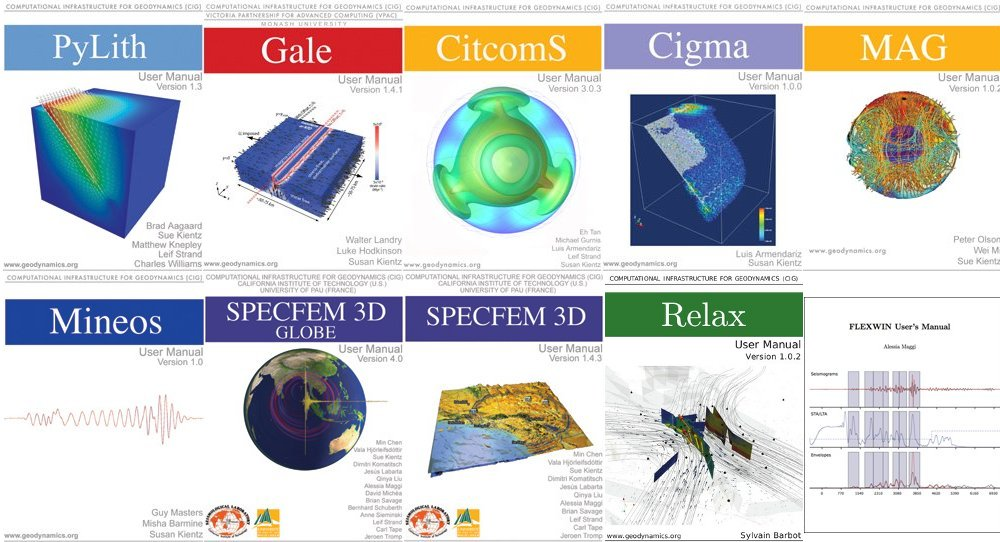
\includegraphics[width=4.5in]{figs/covers}
  \end{center}
  \vfill

\end{frame}

% ------------------------------------------------------------ SLIDE
\begin{frame}
  \frametitle{CIG Software for Crustal Deformation}
  \summary{}

  \begin{itemize}
  \item PyLith
    \begin{itemize}
    \item Solves 2-D and 3-D problems associated with earthquake
      faulting and quasi-static and dynamic viscoelastic deformation
    \item Short-term tectonics where geometry does not change
      significantly
    \end{itemize}
  \item Relax
    \begin{itemize}
    \item Solves 3-D problems associated with earthquake faulting and
      quasi-static viscoelastic deformation
    \item Short-term tectonics in a homogeneous half-space where
      geometry does not change significantly
    \end{itemize}
  \item Gale
    \begin{itemize}
    \item Solves problems in orogenesis, rifting, and subduction,
      including free surfaces with coupling to surface erosion models
    \item Long-term tectonics where geometry changes significantly
    \end{itemize}
  \end{itemize}
 
\end{frame}

 
% ======================================================================
\end{document}


% End of file
